\section{Lektion 20-02-2018}

\begin{enumerate}
	\item Interfaces to CODEC, SPORT and SPI
	\item Sample and Block Processing
	\item Memory and DMA
\end{enumerate}

\begin{mdframed}[style=exampledefault]
\begin{itemize}
	\item ESP 5.1.4 (Memory)
	\item ESP 6.3 (Sample and block processing)
	\item ESP 7.1 (CODEC and SPORT)
	\item ESP 7.2 (DMA)
\end{itemize}
\end{mdframed}

\subsection{Interfaces to CODEC, SPORT and SPI}
Transfer of data between the ADC and memory, within memory spaces, and between memory and peripherals with DMA.

\subsubsection{CODEC}
\begin{itemize}
	\item A CODEC consists of both ADC and DAC with associated analog antialiasing and reconstruction low-pass filters.
	\begin{itemize}
		\item 2 stereo ADC, 3 stereo DAC.
		\begin{itemize}
			\item Operates in 16-, 18-, 20-, or 24-bit resolution.
		\end{itemize}
		\item TDM mode, 48-kHz sampling rate.
		\item I2S mode, 96 kHz sampling rate, only primary channels active.
	\end{itemize}
\end{itemize}

\subsubsection{SPI}
One SPI provides high-speed serial communication of up to SCLK/4. It
interfaces with another processor, data converters, and display.
\begin{itemize}
	\item CODEC setup using SPI interface.
\end{itemize}

\subsubsection{SPORT}
Two synchronous serial ports (SPORT0 and SPORT1) provide high-speed
serial communication with a maximum speed of SCLK/2. This provides an
efficient interface with CODEC.
\begin{itemize}
	\item Receive clock (Internal or External)
	\item Transmission synchronized with CODEC
	\item Buffers to handle Rx and Tx data
	\item I2S mode is standard for stereo channels (L/R)
	\item TDM mode (Time Division Multiplex)
	\item Tansfers 8 channels in every frame
	\item Configuration: bits, DMA, interrupts, bit order
	\begin{itemize}
		\item ESP 7.1.2
	\end{itemize}
\end{itemize}

\subsubsection{I2S}
\begin{itemize}
	\item Three-wire serial	bus standard protocol.
	\item Two time slots for left and right channels.
\end{itemize}
\begin{figure} [H]
	\centering
	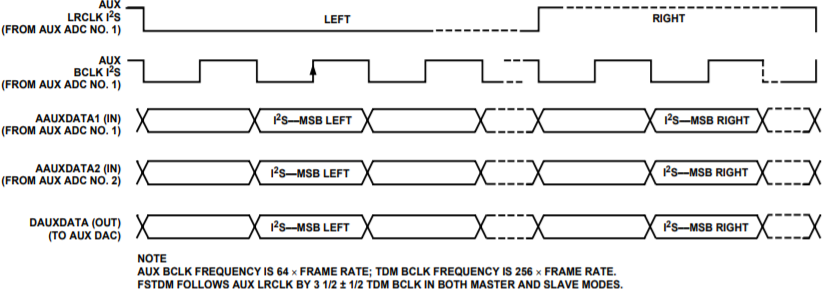
\includegraphics[width=\linewidth]{graphics/21.png}
	\caption{AUX I2S Interface}
	\label{fig:21}
\end{figure}

\subsubsection{TDM}
\begin{itemize}
	\item Time-Division Multiplex Mode.
	\item Two ADC left channels (L0 and L1) and two right channels (R0 and R1) occupy slots \#1, \#2, \#5, and \#6 of ASDATA1.
	\item Six DAC channels occupy the six time slots of DSDATA1.
	\item Special TDM auxiliary mode allows	two external stereo ADCs and one external stereo DAC to be interfaced to form a total of eight input and eight output transfers.
\end{itemize}

\begin{figure} [H]
	\centering
	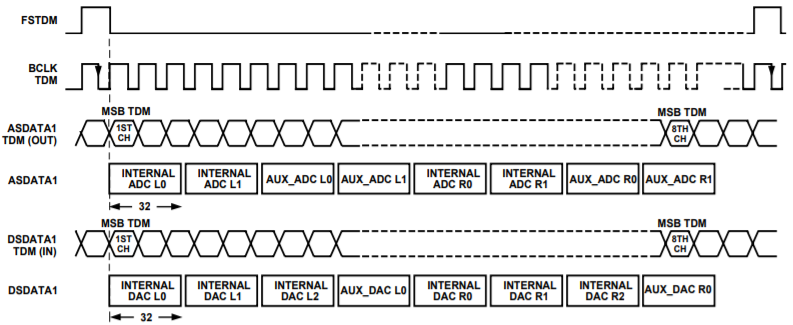
\includegraphics[width=\linewidth]{graphics/20.png}
	\caption{TDM Interface.}
	\label{fig:20}
\end{figure}

\subsection{Sample and Block Processing}
\begin{itemize}
	\item \textbf{Sample-by-Sample Processing}
	\begin{itemize}
		\item Requires that all operations must be completed within the given sampling period.
		\item Latency of processing is the total time from the instant the data sample is read to the time the digital output is written to the memory.
		\begin{itemize}
			\item $T_{in}$ = time needed for the processor to copy current sample from ADC into processor memory. Also includes program access time.
			\item $T_{sp}$ = time needed for processing current data samples. Duration depends on complexity of the algorithm and efficiency of the	program.
			\item $T_{out}$ = time needed to output the processed data to the DAC.
		\end{itemize}
		\item Overall overhead time for sample-by-sample processing is denoted as $T_{os}$.
		\begin{itemize}
			\item Includes $T_{in}$ and $T_{out}$ and response time to interrupt.
		\end{itemize}
		\item Terminated processing before next sample/block. 
		\begin{itemize}
			\item $T_{sp} \leq T_s - T_{os}$
		\end{itemize}
		\item Advantages?
		\begin{itemize}
			\item Predictable processing time ($T_s$).
			\item Delay between input and output within one sample.
			\item Low memory usage for storage will though increase for multichannel applications.
			\item Results are kept current within the sampling period.
		\end{itemize}
		\item Disadvantages?
		\begin{itemize}
			\item Overhead of setup, access, interrupt for every sample.
			\item DSP must be fast enough to complete all task	before the arrival of next input sample.
			\item Not suitable for block based algorithms like Fourier transformation.
		\end{itemize} 
	\end{itemize}
\end{itemize}

\begin{figure} [H]
	\centering
	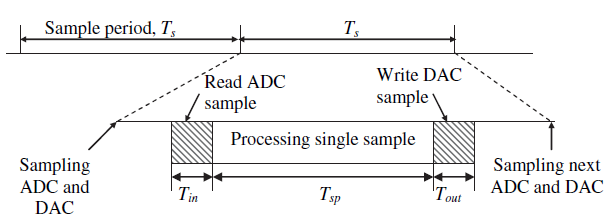
\includegraphics[width=0.8\linewidth]{graphics/19.png}
	\caption{Timing details for sample-by-sample processing mode.}
	\label{fig:19}
\end{figure}

\begin{itemize}
	\item \textbf{Block Processing}
	\begin{itemize}
		\item Samples are gathered in input buffer for N samples received
		\item Interrupt for every sample block of size N
		\item Block delay = $2\cdot N\cdot T_s$
		\item Doublet buffering for input and output samples
		\item DMA used to move data between SPORT and buffers (Sample buffer)
		\newpage \item Advantages?
		\begin{itemize}
			\item Instruction cycle to compute a block of samples is shorter compared to sample-by-sample processing.
		\end{itemize}
		\item Disadvantages?
		\begin{itemize}
			\item Memory of 4 buffers for holding input and output
			data samples.
			\item Block delay $2\cdot N\cdot T_s$.
			\item Complexity in programming switching between buffers.
		\end{itemize}
	\end{itemize}
\end{itemize}

The block processing system starts by sampling the first five input
samples from the ADC to form block \textit{i}. The system continues to sample another five data samples to form block \textit{i + 1}. At the same time, the processor operates on data samples in block \textit{i} and sends the five previously processed samples to the DAC. During the next block period, \textit{i + 2}, another five newer samples are acquired. The processor operates on the data samples in block \textit{i + 1} and outputs the processed data samples in block \textit{i}.

\begin{figure} [H]
	\centering
	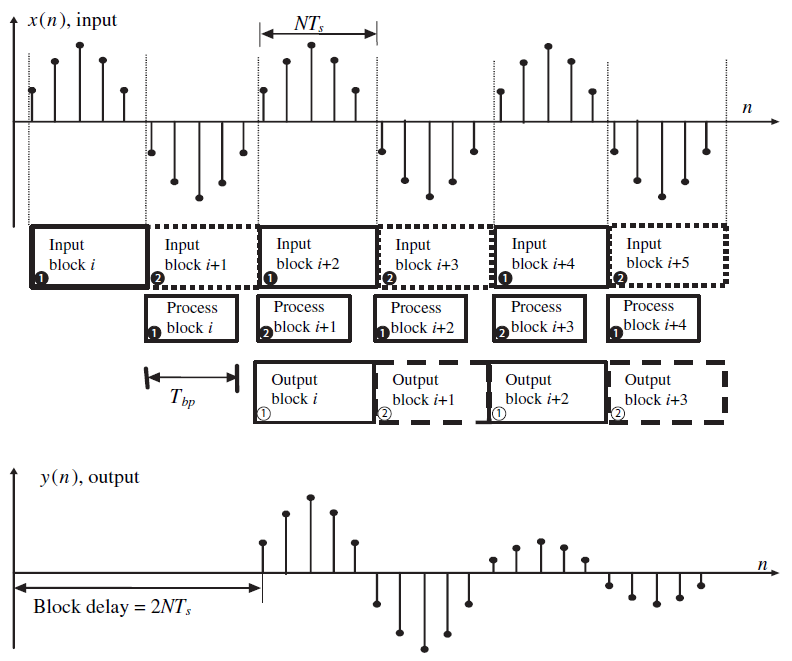
\includegraphics[width=\linewidth]{graphics/18.png}
	\caption{Block processing mode (N = 5).}
	\label{fig:18}
\end{figure}

\subsubsection{Example of Sample-by-Sample Processing}
\begin{minted}{c}
EX_INTERRUPT_HANDLER(Sport0_RX_ISR)
{
// confirm interrupt handling
*pDMA1_IRQ_STATUS = 0x0001;
// Move data from receive buffer to local buffer
// Retrieve all the samples from receive buffer to process buffer
sCh0LeftIn = sDataBufferRX[INTERNAL_ADC_L0];
sCh0RightIn = sDataBufferRX[INTERNAL_ADC_R0];
sCh1LeftIn = sDataBufferRX[INTERNAL_ADC_L1];
sCh1RightIn = sDataBufferRX[INTERNAL_ADC_R1];

Process_Data();

sDataBufferTX[INTERNAL_DAC_L0] = sCh0LeftOut;
sDataBufferTX[INTERNAL_DAC_R0] = sCh0RightOut;
sDataBufferTX[INTERNAL_DAC_L1] = sCh1LeftOut;
sDataBufferTX[INTERNAL_DAC_R1] = sCh1RightOut;
}
\end{minted}

\subsubsection{Example of Block Processing}
\begin{minted}{c}
EX_INTERRUPT_HANDLER(Sport0_RX_ISR)
{
int i;
static short j=0;
// confirm interrupt handling
*pDMA1_IRQ_STATUS = 0x0001;
// Move data from receive buffer to local buffer
for (i = 0; i < INPUT_SIZE; i++)
{
	// Retrieve all the samples from receive buffer to process buffer
	sCh0LeftIn[i] = sDataBufferRX[INTERNAL_ADC_L0+j];
	sCh0RightIn[i] = sDataBufferRX[INTERNAL_ADC_R0+j];
	sCh1LeftIn[i] = sDataBufferRX[INTERNAL_ADC_L1+j];
	sCh1RightIn[i] = sDataBufferRX[INTERNAL_ADC_R1+j];
	// use the builtin circular buffer to update the index
	j = circindex(j, 4, 4*INPUT_SIZE*TOTAL_FRAME);
}
Process_Data();
...
\end{minted}

\subsection{Memory and DMA}
\subsubsection{Memory Types}
\begin{itemize}
	\item L1 Instruction and Data memory
	\begin{itemize}
		\item Blackfin processor supports a hierarchical memory model.
		\item Single-cycle execute and access.
		\item 10's of kBytes - speed $>$ \SI{600}{\mega\hertz} (CCLK).
		\item Transfer	data from memory to registers is arranged in a hierarchy from the slowest (L3 memory) to the fastest (L1 memory).

	\end{itemize}
	\item L3 Extern memory
	\begin{itemize}
		\item External off-chip memory like SDRAM.
		\item Used to hold large program and data.
		\item 100's of Mbytes – speed $<$ \SI{133}{\mega\hertz}  (SCLK).
	\end{itemize}
\end{itemize}

\begin{figure} [H]
	\centering
	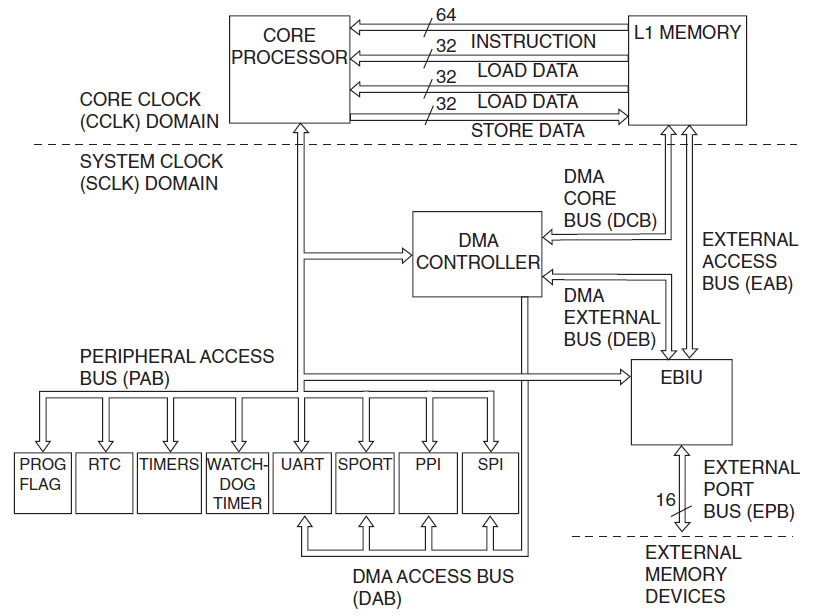
\includegraphics[width=\linewidth]{graphics/17.png}
	\caption{BF533 processor memory architecture.}
	\label{fig:17}
\end{figure}

\subsubsection{DMA Modes}
\begin{itemize}
	\item Stop Mode
	\begin{itemize}
		\item Stopped after transfer is completed
	\end{itemize}
	\item Auto Buffer Mode
	\begin{itemize}
		\item Automatic restart when data transfer is completed
	\end{itemize}
	\item Descriptor Mode
	\begin{itemize}
		\item Descriptor list in memory that specifies the next
		data transfer (source and destination address).
		\item Descriptor is automatic read by the DMA controller.
	\end{itemize}
\end{itemize}

\subsubsection{DMA Initialization}
\begin{itemize}
	\item Start address
	\item Peripheral device map
	\begin{itemize}
		\item \mintinline{c}{DMA1_PERIPHERAL_MAP = 0x1000; // channel 1 for SPORT0 RX}
		\item \mintinline{c}{DMA2_PERIPHERAL_MAP = 0x2000; // channel 2 for SPORT0 TX}
	\end{itemize}
	\item Configuration
	\begin{itemize}
		\item Set DMA channel 1 for autobuffer mode, enable data interrupt,
		retain DMA buffer, 1D DMA using 16-bit transfers, DMA is a memory write, and DMA channel 1 is not enabled.
		\begin{itemize}
			\item \mintinline{c}{DMA1_CONFIG = 0001 0000 1000 0110b}
		\end{itemize}
		\item Set DMA channel 2 for autobuffer mode, disable data interrupt,
		retain DMA buffer, 1D DMA using 16-bit transfers, DMA is a memory
		read, and DMA channel 2 is not enabled.
		\begin{itemize}
			\item \mintinline{c}{DMA2_CONFIG = 0001 0000 0000 0100b}
		\end{itemize}
	\end{itemize} 
	\item Count (X,Y)
	\item Modify (X,Y)
\end{itemize}
